Segundo \cite{gil2002elaborar}, a pesquisa experimental consiste na definição de um objeto de estudo, na seleção de variáveis capazes de influenciá-lo e na determinação de formas de controle e observação dos efeitos produzidos por essas variáveis. Com base nessa definição, o presente trabalho caracteriza-se como uma pesquisa de natureza experimental, uma vez que modelos de tradução automática neural baseados na arquitetura Transformer serão comparados e submetidos a diferentes cenários e bases de dados.

Além disso, de acordo com \cite{da2002apostila}, a pesquisa quantitativa utiliza linguagem matemática para descrever fenômenos e analisar relações entre variáveis. Nesse contexto, este trabalho também possui caráter quantitativo, pois os modelos serão avaliados por meio de métricas como BLEU, BERTScore e chrF, bem como por medidas de eficiência computacional, obtidas a partir de experimentos controlados.


\section{Modelos}

Nesta seção são descritas as principais características dos modelos selecionados para comparação na tarefa de tradução automática, incluindo informações como tamanho, finalidade e forma de acesso.

A seguir, são apresentados os modelos utilizados neste trabalho, bem como suas respectivas configurações e locais para obtenção:

\begin{itemize}
    \item \textbf{MarianMT}: O modelo utilizado será o \textit{opus-mt-tc-big-en-pt}, com aproximadamente 0,2 bilhões de parâmetros. Trata-se de um modelo específico para tradução do inglês para o português. O seguinte \href{https://huggingface.co/Helsinki-NLP/opus-mt-tc-big-en-pt}{link} direciona para a plataforma \textit{Hugging Face}, onde o modelo pode ser obtido para uso local.

    \item \textbf{M2M-100}: O modelo utilizado será o \textit{m2m100\_418M}, com aproximadamente 0,4 bilhões de parâmetros. Diferentemente do MarianMT, este modelo não requer a seleção de um par específico de línguas, pois foi projetado para tradução direta entre múltiplos idiomas. O seguinte \href{https://huggingface.co/facebook/m2m100_418M}{link} redireciona para a plataforma \textit{Hugging Face}, onde o modelo pode ser obtido para uso local.

    \item \textbf{NLLB}: O modelo utilizado será o \textit{nllb-200-distilled-600M}, com aproximadamente 0,6 bilhões de parâmetros. Assim como o M2M-100, este modelo permite tradução direta entre múltiplas línguas, sem a necessidade de uma língua intermediária. O seguinte \href{https://huggingface.co/facebook/nllb-200-distilled-600M}{link} redireciona para a plataforma \textit{Hugging Face}, onde o modelo pode ser obtido para uso local.

\end{itemize}

\section{Tipos de texto}

Nesta seção são definidos os tipos de texto utilizados na avaliação dos modelos de tradução automática.

Os textos foram organizados em quatro categorias, considerando o tamanho e o domínio do conteúdo, conforme descrito a seguir:

\begin{itemize}
    \item \textbf{Textos curtos}: textos com até 15 palavras de domínio geral;
    
    \item \textbf{Textos longos}: textos com mais de 15 palavras de domínio geral;

    \item \textbf{Textos gerais}: textos curtos e longos de domínio geral, incluindo conversas cotidianas, diálogos e conteúdos sem especialização técnica, obtidos através de bases de dados públicas;

    \item \textbf{Textos específicos}: textos curtos e longos associados a domínios especializados, como medicina, engenharia e nutrição, também obtidos a partir de bases de dados públicas.

\end{itemize}


\section{Métricas de Avaliação}

Nesta seção tem como objetivo apresentar as ferramentas utilizadas para o cálculo das métricas BLEU, BERTScore e chrF e avaliação das traduções geradas pelos modelos.

\subsection{BLEU}

O cálculo da métrica BLEU, após a geração da tradução pelo modelo, será realizado utilizando a biblioteca da linguagem Python denominada NLTK (\textit{Natural Language Toolkit}). Essa biblioteca disponibiliza diversas funcionalidades voltadas ao processamento de linguagem natural, incluindo a função \textit{sentence\_bleu}, utilizada para calcular o valor da métrica BLEU a nível de sentença.

Essa função recebe como entrada uma ou mais sentenças de referência e a sentença gerada pelo modelo, retornando um valor numérico que representa o grau de similaridade entre elas com base em n-gramas.

Além disso, será utilizado um método de suavização (\textit{smoothing}) para evitar valores nulos em casos de baixa sobreposição entre os n-gramas da sentença gerada e da referência.

Abaixo é apresentado um exemplo de cálculo da métrica BLEU utilizando a função \textit{sentence\_bleu} da biblioteca NLTK:
\\
\\
\\
\\
\\
\\
\\
\begin{listing}
\begin{python}
from nltk.translate.bleu_score import sentence_bleu, SmoothingFunction

referencia = [['Uma', 'raposa', 'pula', 'sobre', 'o', 'cachorro', '.']]
geradoPeloModelo = ['Uma', 'pula','raposa', 'sobre', 'o', 'cachorro', ',']

smooth = SmoothingFunction().method1

print(sentence_bleu(referencia, geradoPeloModelo, smoothing_function=smooth))
\end{python}
\caption{Exemplo de cálculo da métrica BLEU com NLTK}
\label{code:bleu_example}
\end{listing}

\subsection{BERTScore}

O cálculo da métrica BERTScore será realizado utilizando a biblioteca da linguagem Python denominada \textit{bert-score}. Essa biblioteca permite calcular a similaridade entre sentenças por meio da comparação de \textit{embeddings} contextuais gerados a partir de modelos pré-treinados.

A função \textit{score} é responsável por receber como entrada a sentença gerada pelo modelo e a sentença de referência, retornando três medidas principais: precisão, revocação e F1-score.Para este trabalho, será utilizado o F1-score médio como medida final do BERTScore, por representar um equilíbrio entre precisão e revocação.

Abaixo é apresentado um exemplo de cálculo da métrica BERTScore utilizando a função \textit{score} da biblioteca \textit{bert-score}:

\begin{listing}
\begin{python}
from bert_score import score

geradoPeloModelo = ["O tempo esta congelante hoje."]
referencia = ["Hoje esta frio."]

PRECISAO, REVOCACAO, F1_SCORE = score(geradoPeloModelo, referencia, lang="pt", verbose=True)

print(F1_SCORE.mean())

\end{python}
\caption{Exemplo de cálculo da métrica BERTScore com a biblioteca bert-score}
\label{code:bleu_example}
\end{listing}

\subsection{chrF}

Para o cálculo da metrica chrF será realizada utilizada a biblioteca da linguagem python (\textit{sacrebleu}). Essa biblioteca possui funções que realizam o cálculo de métricas para avaliação de traduções automáticas, e dentre elas a função (\textit{sentence\_chrf}), cujo objetivo é realizar o cálculo da métrica chrF dado a sequência gerada pelo modelo e a sequência de referência.


A função (\textit{sentence\_chrf}) recebe dois argumentos, o primeiro sendo a sequência gerada pelo modelo, já o segundo argumento, a sequência de referência. Como resposta, a função retorna um valor entre 0 e 100, indicando o valor da métrica chrF

Abaixo é apresentado um exemplo de cálculo da métrica chrF utilizando a função \textit{sentence\_chrf} da biblioteca \textit{sacrebleu}:
\\
\begin{listing}
\begin{python}
import sacrebleu

geradoPeloModelo = "The cat is on the mat."
referencia = ["The cat is on the mat."]

chrf = sacrebleu.sentence_chrf(geradoPeloModelo, referencia)

print(chrf)

\end{python}
\caption{Exemplo de cálculo da métrica chrF com a biblioteca sacrebleu}
\label{code:bleu_example}
\end{listing}

\section{Ambiente Computacional}

Com o objetivo de garantir um ambiente controlado e uniforme para a comparação entre os modelos de tradução, optou-se pela utilização de um ambiente virtual em nuvem (\textit{cloud}) para execução dos experimentos.A plataforma escolhida foi a \textbf{DigitalOcean}, devido à disponibilidade de instâncias com cobrança por hora e oferta de máquinas com alto desempenho, o que possibilita maior flexibilidade na execução dos testes.

A Tabela abaixo apresenta as especificações da máquina virtual utilizada nos experimentos:

\begin{table}[H]
\centering
\begin{tabular}{ |p{3cm}|p{3cm}|p{3cm}|p{3cm}| }
\hline
\multicolumn{1}{|p{3cm}|}{\centering\textbf{Memória RAM}} & \multicolumn{1}{p{3cm}|}{\centering\textbf{Núcleos (vCPU)}} & \multicolumn{1}{p{3cm}|}{\centering\textbf{Transferência de dados}} & \multicolumn{1}{p{3cm}|}{\centering\textbf{Armazenamento}} \\
\hline
\multicolumn{1}{|p{3cm}|}{\centering 16 GB} & \multicolumn{1}{p{3cm}|}{\centering 8 vCPUs} & \multicolumn{1}{p{3cm}|}{\centering 6 TB} & \multicolumn{1}{p{3cm}|}{\centering 100 GB} \\
\hline
\end{tabular}
\caption{Especificações da máquina virtual utilizada}
\label{tab:ambiente_computacional}
\end{table}

Cabe destacar que, por se tratar de um ambiente virtualizado, informações detalhadas sobre o hardware físico, como modelo do processador ou tipo de memória, não são explicitamente fornecidas pela plataforma. Isso ocorre porque a instância virtual pode ser alocada dinamicamente sobre diferentes máquinas físicas, dependendo da disponibilidade no momento da criação.

\section{Procedimento de Execução}

\begin{figure}[H]
    \centering
    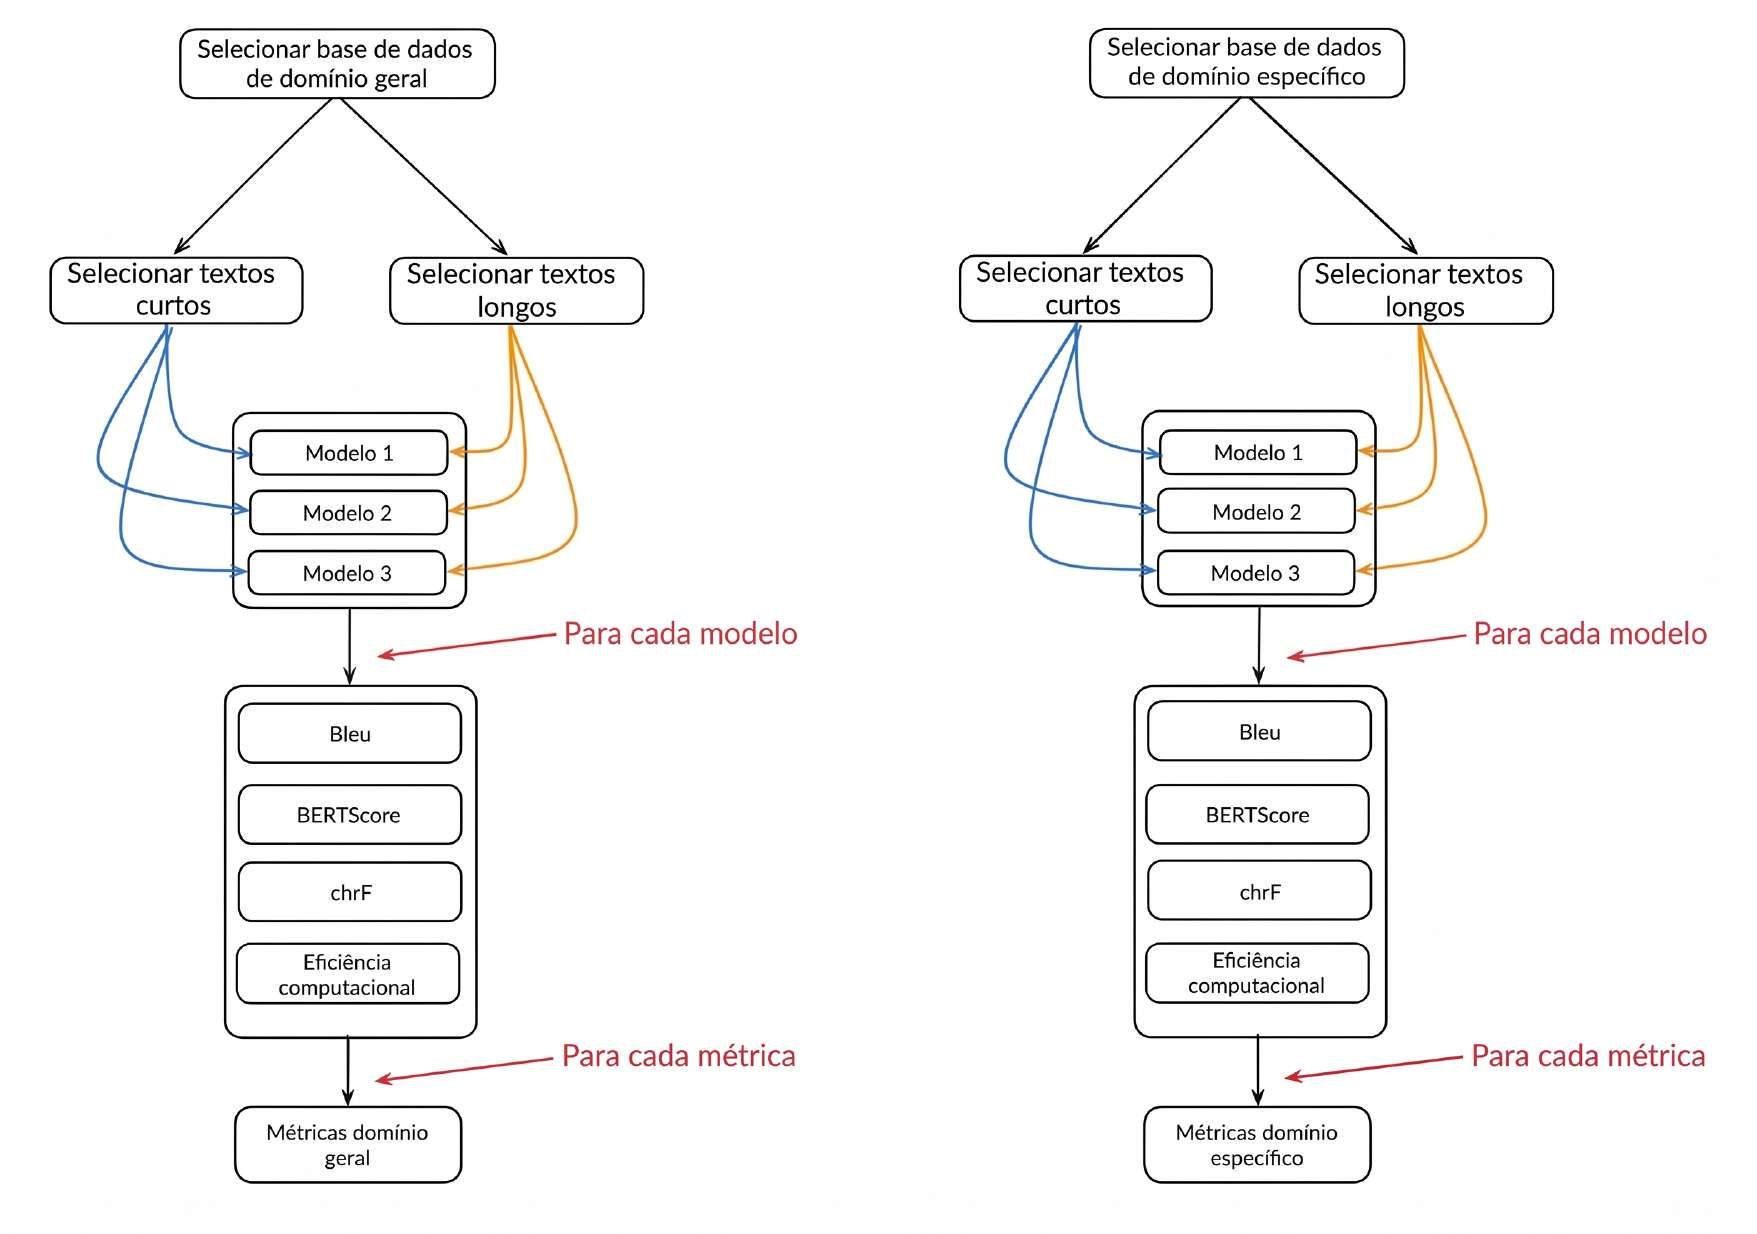
\includegraphics[height=0.7\textwidth]{Imagens/procedure-general.pdf}    \caption{\label{fig:procedimento} Procedimento}
    \legend{Fonte: autor}
\end{figure}

\section{Desempenho Computacional}

Nesta seção são descritas as métricas e ferramentas utilizadas para avaliação da eficiência computacional dos modelos de tradução, considerando principalmente o uso de CPU, tempo de execução e consumo de memória RAM.

\subsection{Uso de CPU e Tempo de Execução}

Neste experimento, serão considerados dois indicadores principais relacionados à CPU: o tempo médio de execução e o uso médio de CPU durante a tarefa de tradução.

Para a medição do tempo de execução, será utilizada a ferramenta de linha de comando \textit{hyperfine}. Essa ferramenta é amplamente utilizada para a realização de benchmarks, permitindo medir o tempo total, média e desvio padrão de execução de um programa ao longo de múltiplas execuções.

Abaixo é apresentado um exemplo de uso da ferramenta \textit{hyperfine}:

\begin{listing}
\begin{python}
hyperfine 'python3 script.py'
\end{python}
\caption{Exemplo de uso da ferramenta \textit{hyperfine}}
\label{code:hyperfine}
\end{listing}

Para a medição do uso médio de CPU durante a execução dos modelos, será utilizada a ferramenta \textit{pidstat}, nativa de sistemas operacionais Linux. Essa ferramenta permite coletar estatísticas detalhadas sobre o uso de recursos por processos individuais.

A seguir, um exemplo de utilização da ferramenta \textit{pidstat}:

\begin{listing}
\begin{python}
pidstat -u -e python3 test.py
\end{python}
\caption{Exemplo de uso da ferramenta \textit{pidstat}}
\label{code:pidstat}
\end{listing}

As principais flags utilizadas são:

\begin{itemize}
    \item \textbf{-u}: exibe estatísticas de utilização da CPU;
    \item \textbf{-e}: executa o comando especificado e monitora seu consumo de recursos.
\end{itemize}

\subsection{Consumo de Memória RAM}

Para a análise de memória RAM, serão considerados dois indicadores: o uso médio e o uso máximo (pico) durante a execução da tarefa de tradução. O uso médio de memória será obtido por meio da ferramenta \textit{pidstat}, utilizando a flag \textit{-r}, que permite monitorar o consumo de memória ao longo da execução do processo.

Já o uso máximo de memória (pico) será medido utilizando a ferramenta \textit{/usr/bin/time}, também disponível em sistemas Linux. Essa ferramenta fornece informações detalhadas sobre a execução de programas, incluindo o consumo máximo de memória.

Abaixo é apresentado um exemplo de uso da ferramenta \textit{time}:

\begin{listing}
\begin{python}
/usr/bin/time -v python3 script.py
\end{python}
\caption{Exemplo de uso da ferramenta \textit{time}}
\label{code:time}
\end{listing}

A flag \textit{-v} permite a exibição de informações detalhadas, incluindo o valor de memória máxima utilizada durante a execução do programa.